\documentclass[9pt,conference]{IEEEtran}
\IEEEoverridecommandlockouts
% The preceding line is only needed to identify funding in the first footnote. If that is unneeded, please comment it out.
%Template version as of 6/27/2024

\usepackage{cite}
\usepackage{amsmath,amssymb,amsfonts}
\usepackage{algorithmic}
\usepackage{graphicx}
\usepackage{textcomp}
\usepackage{xcolor}
\def\BibTeX{{\rm B\kern-.05em{\sc i\kern-.025em b}\kern-.08em
    T\kern-.1667em\lower.7ex\hbox{E}\kern-.125emX}}

\usepackage[main=german]{babel}
\usepackage[german]{cleveref}

% for compatibility with natbib for \citeauthor etc: https://tex.stackexchange.com/a/202964
\bibliographystyle{IEEEtranN}
\usepackage[numbers]{natbib}

\begin{document}

\title{Memento Pattern\\
}

\author{\IEEEauthorblockN{1\textsuperscript{st} Herrmann, Axel}
\IEEEauthorblockA{\textit{Knowledge Foundation @ Reutlingen University} \\
Stuttgart, Germany \\
axel.herrmann@weiterbildung-reutlingen-university.de}
}

\maketitle

\section{Einleitung}
Entwurfsmuster bieten bewährte Lösungen für häufige Designprobleme in der Softwareentwicklung, fördern Wiederverwendbarkeit und Flexibilität des Codes und erleichtern die Kommunikation im Team durch gemeinsame Begriffe. 
Sie helfen Entwicklern, komplexe Probleme effizienter zu lösen und robuste, wartbare Software zu erstellen. 
Sehr bekannte Entwurfsmuster sind die von \Citet{gamma1993design} vorgestellten Patterns, welche in Erzeugungsmuster, Strukturmuster und Verhaltensmuster unterteilt werden.
Das Memento Pattern ist eines dieser Entwurfsmuster, welches als Verhaltensmuster eingeordnet wird.

\section{Kontext}
In vielen Anwendungen gehen Nutzer heutzutage davon aus, dass vorherige Zustände wiederhergestellt werden können. Beispiele finden sich in Texteditoren mit der \glqq{}Undo\grqq{}-Funktion, in Computerspielen mit speicherbaren Spielständen oder in der Datenbankentwicklung, wo Transaktionen zurückgerollt werden können. Solche Anforderungen können durch die Speicherung von Zustandsinformationen eines Objekts umgesetzt werden.
Um den Zustand eines Objekts zu speichern und diesen zu einem späteren Zeitpunkt potentiell wiederherstellen zu können, muss der zustandsrelevante Teil des Objekts kopiert und abgespeichert werden.
Dieser Prozess dessen ist non-trivial, da eine einfache Kopie das Objekts gegen das Prinzip der Kapselung verstößt.
Kapselung ist wichtig, um die Integrität des Zustands zu schützen \cite{encapsulation}.
Bei Zugriff anderer Objekte auf die Zustandsinformationen können unerwünschte Nebeneffekte auftreten.
Um also gleichzeitig von der Qualitätserhöhung von Software durch eingehaltene Kapselung und umgesetzten Rollback-Möglichkeiten zu profitieren, sollte eine klare Methodik verwendet werden, die diese beiden, auf den ersten Blick widersprüchlich wirkenden Forderungen, vereint.

\section{Ansatz}
Dieses Problem versucht das Memento Pattern, vorgestellt von \Citet{gamma1993design}, und auch \emph{Snapshot} genannt \cite{refactoring-guru}, zu lösen.
Die Idee dabei ist, dass das zu speichernde Objekt, der \emph{Originator}, eine Momentaufnahme seines Zustands in einem separaten Objekt, welches \emph{Memento} genannt wird, speichert.
Ausgelöst wird dieses Verhalten durch ein weiteres Objekt, das \emph{Caretaker} genannt wird.
Dieses verwaltet eine Historie von Momentaufnahmen und kann sie später verwenden, um den Zustand des Originators wiederherzustellen.
Der Fokus des Entwurfsmusters liegt unter anderem darauf, die Kapselung des Originator-Objekts zu bewahren, indem der Caretaker keinen direkten Zugriff auf die internen Details erhält \cite{geeksforgeeks}.
Dadurch wird eine klare Trennung zwischen den Rollen des Originators und des Caretakers gewährleistet.
Für das Erreichen dieses Zielzustands gibt es nicht nur einen offensichtlichen besten Lösungsweg, sondern mehrere Implementierungsansätze, abhängig von den Anforderungen der jeweiligen Anwendung.

\section{Implementierung}
Je nach Programmiersprache und gewünschter Sicherheit der Einhaltung der Kapselung gibt es verschiedene konkrete Umsetzungsmöglichkeiten des Patterns.
In den folgenden Abschnitten werden drei gängige Ansätze nach \cite{refactoring-guru} vorgestellt.

\subsection{Verschachtelte Klasse}
Eine Möglichkeit der Implementierung liegt in der Nutzung des Prinzips der verschachtelten Klassen, welches in einigen Programmiersprachen wie Java, C++ und C\# möglich ist.
\begin{figure}[htbp]
	\centerline{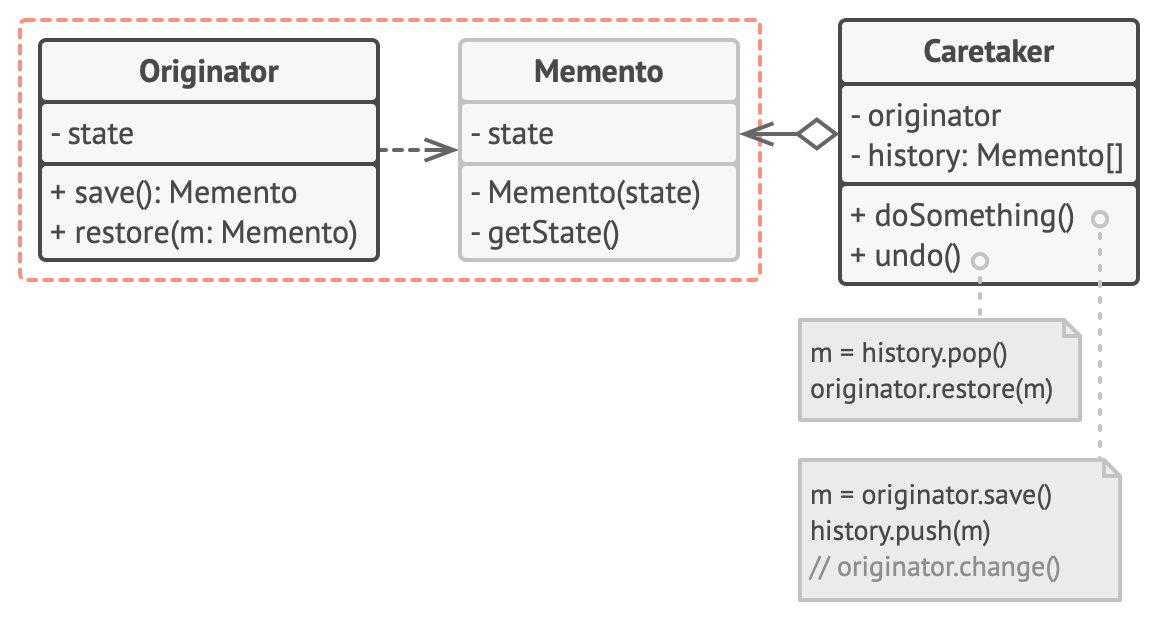
\includegraphics[width=0.4\textwidth]{figures/nested-class.png}}
	\caption{Implementierung des Memento Patterns nach \cite{refactoring-guru} mit Nutzung einer verschachtelten Klasse.}
	\label{fig:nested-class}
\end{figure}
Bei diesem Ansatz wird die Memento-Klasse als innere Klasse innerhalb des Originators definiert.
Der Originator besitzt dadurch direkten Zugriff auf die privaten Felder und Methoden des Mementos, was die Implementierung vereinfacht.
Die Kapselung wird aufrechterhalten, da die Memento-Klasse für den Caretaker und andere externe Objekte vollständig verborgen bleibt.
Von außen sieht die interne Struktur des Mementos wie eine Blackbox aus und lediglich bewusst zugängig gemachte Methoden können verwendet werden.
Typischerweise können Caretaker so beispielsweise die Zeitpunkte oder Namen der Mementos einsehen.

Ein praktisches Beispiel ist die Speicherung von Spielständen in einem Videospiel.
Der Spielstand (Memento) wird in der Engine (Originator) als innere Klasse definiert.
Dadurch kann die Engine den Zustand direkt speichern und wiederherstellen, während der Caretaker, z. B. eine Benutzeroberfläche, lediglich den Spielstand verwaltet, ohne Details darüber zu kennen.
Dort kann dem Nutzer dann der Name des Spielstands oder der Zeitpunkt der letzten Speicherung angezeigt werden.

Dieser Ansatz eignet sich besonders dann, wenn die Sprache eine einfache Unterstützung für innere Klassen bietet und die Anforderungen an die Kapselung hoch sind.
Ein Nachteil kann jedoch die enge Kopplung zwischen Originator und Memento sein, da die beiden Klassen in diesem Modell untrennbar verbunden sind.

\subsection{Zwischengeschaltetes Interface}
Eine alternative Implementierung nutzt ein Interface, das die Interaktion zwischen dem Caretaker und dem Memento regelt.
\begin{figure}[htbp]
	\centerline{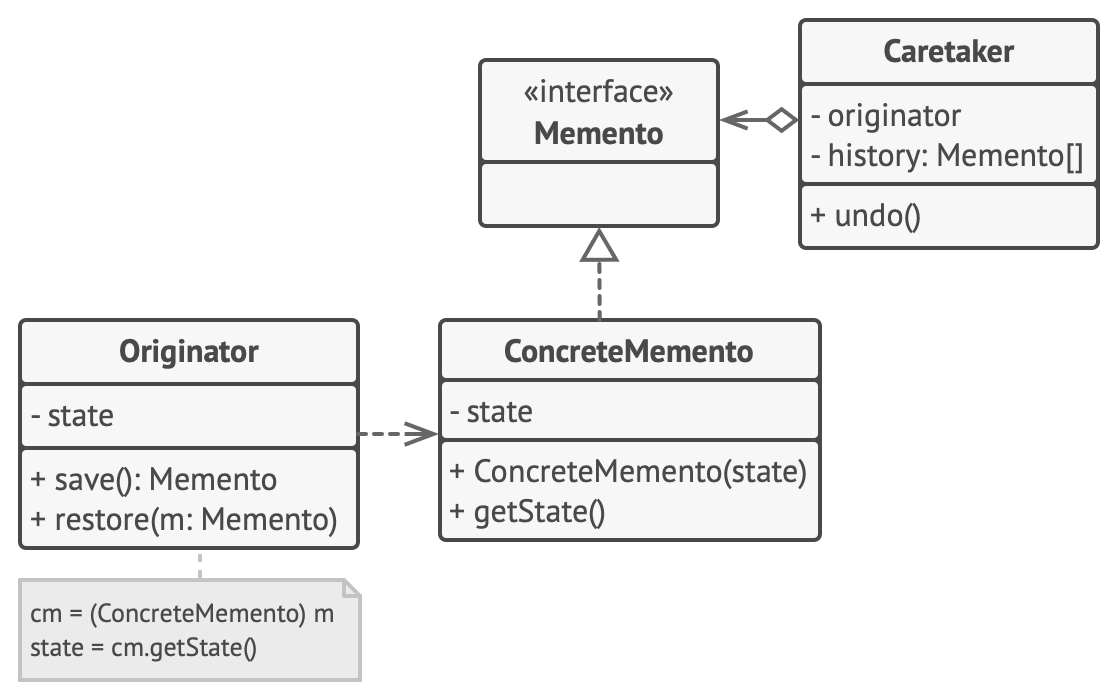
\includegraphics[width=0.4\textwidth]{figures/Intermediate-interface.png}}
	\caption{Implementierung des Memento Patterns nach \cite{refactoring-guru} mit Nutzung eines zwischengeschalteten Interfaces.}
	\label{fig:intermediate-interface}
\end{figure}
Dabei regelt das Prinzip der Polymorphie den Zugriff auf den internen Zustand des Mementos.
Das Memento ist nämlich in ein Interface, welches lediglich die öffentlich zugänglichen Methoden definiert und eine \emph{ConcreteMemento}-Klasse, welche dieses Interface implementiert, aufgeteilt.
Die Idee ist, dass externe Objekte wie Caretaker das Memento lediglich als Interface kennen und somit nur die öffentlich einsehbaren Attribute und Methoden verwenden können, wohingegen der Originator die Mementos als ConcreteMemento referenziert. 

Dieser Ansatz bietet mehrere Vorteile.
Zum einen wird die Interaktion zwischen den Klassen klar definiert und getrennt, was die Wartbarkeit des Codes verbessert.
Zum anderen können mehrere unterschiedliche Memento-Typen verwendet werden, solange sie das gleiche Interface implementieren.
Das ist nützlich, wenn ein System mehrere verschiedene Zustände oder Datenarten speichern und wiederherstellen muss.

Ein Beispiel ist ein Texteditor, der unterschiedliche Memento-Typen für Textformatierungen, Cursorpositionen oder geöffnete Tabs verwendet.
Der Caretaker muss in diesem Fall nur wissen, wie man das Interface verwendet, während der Originator die genaue Funktionsweise kontrolliert.
Ein Nachteil dieser Methode ist die erhöhte Komplexität, da zusätzliche Klassen und Schnittstellen definiert werden müssen.
Für kleine Projekte kann das die Übersichtlichkeit verringern und zu unnötigem Overhead führen.

\subsection{Strikte Kapselung}
Ein Ansatz zur maximalen Wahrung der Kapselung ist die vollständige Trennung von Originator und Caretaker, sodass der Caretaker ausschließlich mit abstrahierten oder anonymisierten Mementos arbeitet.
\begin{figure}[htbp]
	\centerline{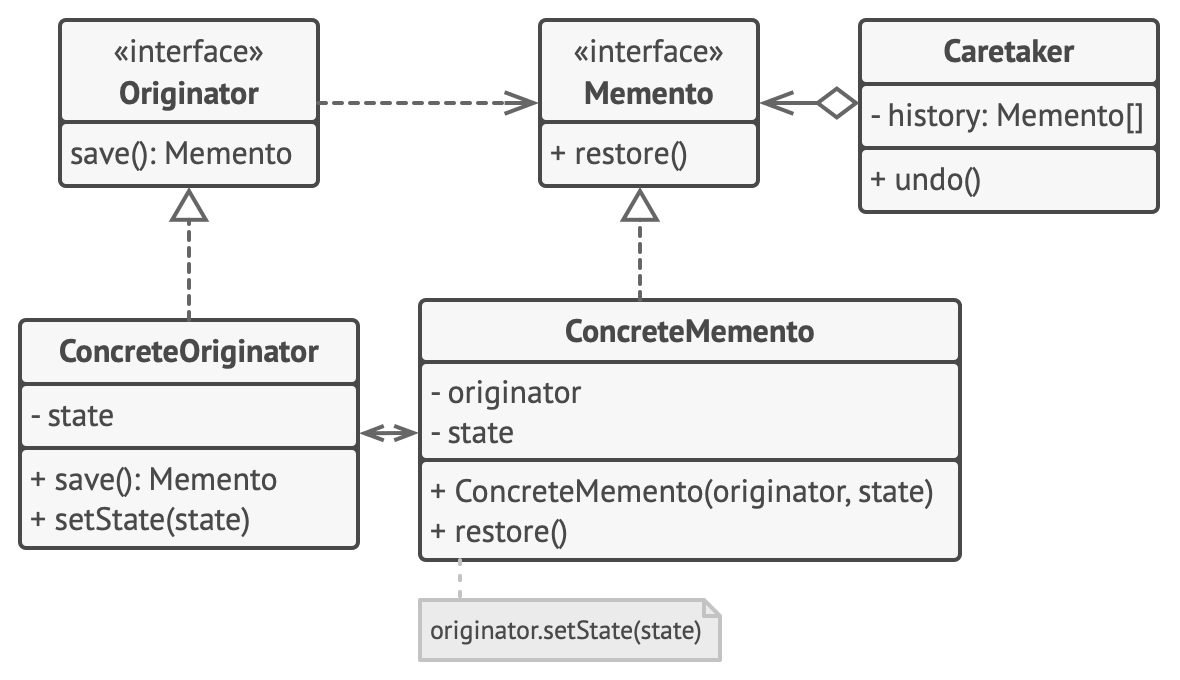
\includegraphics[width=0.4\textwidth]{figures/strict-encapsulation.png}}
	\caption{Implementierung des Memento Patterns nach \cite{refactoring-guru} mit starker Absicherung der Kapselung.}
	\label{fig:strict-implementation}
\end{figure}
Diese Art der Implementierung ermöglicht die Wiederverwendung eines Originator- und Memento-Interfaces für mehrerer Typen der beiden.
Dabei würde jede konkrete Implementierung eines Originators mit einer Memento-Implementierung verknüpft sein.
So sind externe Objekte wie Caretaker explizit daran gehindert, den Zustand der Mementos zu betrachten oder verändern.
Außerdem ist die Caretaker-Klasse in dieser Version unabhängig vom Originator, da das Memento-Interface die restore-Funktion anbietet.
Originator und Memento sind in dieser Implementierung explizit auf Objektebene gekoppelt, indem bei der Erstellung von Mementos das Originator Objekt mit übergeben wird.
Dadurch kann das Memento den Zustand des Originators zurücksetzen, wenn dieser passende Zugriffsmethoden definiert hat.

Ein potenzieller Nachteil dieser Methode ist der zusätzliche Implementierungsaufwand.
Schon an der Größe der Übersicht ist zu sehen, dass diese Implementierung konzeptionell im kompliziertesten ist.
In vielen Fällen wird vermutlich eine der vorherigen beiden Methoden ebenfalls ausreichende Sicherheit der Kapselung bei weniger Aufwand bieten.

\section{Diskussion}

Das beschriebene Vorgehen nach Memento Pattern kann wirksam genutzt werden, um den früheren Zustand einer Applikation durch das Erstellen eines Snapshots wiederherzustellen.
Besonders im Fokus des Patterns liegt dabei das Aufrechterhalten der Kapselung des Originator Objekts, was zugleich der große Vorteil bei Verwendung des Entwurfsmusters ist.
Außerdem unterstützt das Pattern das Prinzip der \emph{Separation of Concerns}, indem es die Zustandsverwaltung vom Originator entkoppelt \cite{geeksforgeeks}.

Zugleich bringt das Muster allerdings auch Nachteile mit sich.
Mit der Speicherung mehrerer Zustände geht natürlich, abhängig von der Größe der Zustände und auch der Anzahl der gespeicherten Zustände, mitunter eine nicht unerhebliche Hauptspeicher-Last einher.
Außerdem ist eine große Motivation für das Memento Pattern der Wunsch nach Kapselung, welcher jedoch vor allem in dynamischen Programmiersprachen nicht vollkommen garantiert werden kann.
Als Beispiel dafür kann Typescript genannt werden, wobei zwar zur Compile-Zeit ein Zugriff auf private Attribute verhindert werden kann, jedoch durch die Kompilierung zu Javascript zur Laufzeit keine Versicherungen gemacht werden können.
Dagegen könnte allerdings argumentiert werden, dass dieses Problem bei der Wahl einer solchen Programmiersprache im Allgemeinen bekannt ist und akzeptiert werden muss.
Abgesehen davon wäre bei Lösung des Memento Patterns über Polymorphie auch in statisch typisierten Programmiersprachen eine Konvertierung möglich, durch die der Kapselungsmechanismus umgangen werden könnte.

\section{Fazit}

Abschließend lässt sich sagen, dass das Memento Pattern eine gute Möglichkeit bietet, auf eine praktische Art und Weise \glqq{}Undo\grqq{}-Funktionalität zu einem Programm hinzuzufügen und zugleich eine hohe Code-Qualität zu wahren, indem Kapselung trotzdem nicht verletzt wird.
Die Schwierigkeit in der Anwendung sollte allerdings nicht unterschätzt werden, da es nicht nur eine konkrete Implementierungsmöglichkeit gibt und allgemein die Code-Komplexität erhöht wird.
Zuletzt sollte nicht vergessen werden, dass die genannten Implementierungsmethoden die Kapselung nicht mit voller Sicherheit gewährleisten können.

\bibliography{IEEEabrv,bibliography}

\end{document}
